% Chương 6
\chapter[\MakeUppercase{Cài đặt, triển khai và kết quả hệ thống}]{Cài đặt, triển khai và kết quả hệ thống}
\label{ch:chuong6}

\section{Yêu cầu hệ thống}

Hệ thống chạy dưới dạng nhiều tiến trình: giao diện Next.js, sáu service và bảy container hạ tầng. Mỗi tiến trình mở một cổng riêng nên có thể khởi động, dừng và xem nhật ký độc lập. Bảng~\ref{tab:cong-cu} liệt kê công cụ cần cài đặt; Bảng~\ref{tab:cong} liệt kê cổng mặc định của từng thành phần.

\begin{table}[H]
  \centering
  \caption{Công cụ cài đặt và phiên bản dùng trong đồ án}\label{tab:cong-cu}
  \begin{singlespace}
  \begin{tabular}{|>{\raggedright\arraybackslash}p{0.28\textwidth}|>{\raggedright\arraybackslash}p{0.22\textwidth}|>{\raggedright\arraybackslash}p{0.4\textwidth}|}
  \hline
  \textbf{Công cụ} & \textbf{Phiên bản} & \textbf{Vai trò} \\ \hline
  Docker Engine kèm Compose & Compose v2 & Chạy bảy container hạ tầng \\ \hline
  JDK & 21 & Build và chạy bốn service Spring Boot \\ \hline
  Node.js, pnpm & Node 20 trở lên, pnpm 11.9.0 & Build và chạy giao diện Next.js \\ \hline
  Python, uv & 3.12 & Tạo môi trường ảo và chạy hai service Python \\ \hline
  Trình duyệt & Chrome, Edge hoặc Firefox bản mới & Kiểm thử giao diện và gọi video WebRTC \\ \hline
  \end{tabular}
  \end{singlespace}
\end{table}

Khi phát triển, bảy container hạ tầng, sáu service, tiến trình worker và giao diện chạy đồng thời trên một máy. Mô hình CNN chạy trên CPU vì service AI dùng gói \texttt{pytorch-cpu}; đồ án không yêu cầu GPU. Dữ liệu của Neo4j, Qdrant và PostgreSQL nằm trong volume Docker nên dung lượng đĩa tăng theo số sách đã số hóa.
% TODO: đo mức tiêu thụ RAM/CPU khi chạy đồng thời cả cụm để bổ sung yêu cầu tối thiểu.

\begin{table}[H]
  \centering
  \caption{Cổng mặc định của các thành phần}\label{tab:cong}
  \begin{singlespace}
  \begin{tabular}{|>{\raggedright\arraybackslash}p{0.36\textwidth}|>{\raggedright\arraybackslash}p{0.16\textwidth}|>{\raggedright\arraybackslash}p{0.38\textwidth}|}
  \hline
  \textbf{Thành phần} & \textbf{Cổng} & \textbf{Ghi chú} \\ \hline
  Giao diện Next.js & 3010 & Điểm vào của người dùng \\ \hline
  API Gateway & 3040 & Định tuyến \texttt{/api/v1/**} tới các service \\ \hline
  Dịch vụ định danh & 3051 & Đăng ký, đăng nhập, hồ sơ \\ \hline
  Dịch vụ tư vấn & 3052 & Hội thoại, tin nhắn, kênh theo dõi \\ \hline
  Dịch vụ lâm sàng & 3053 & Lịch hẹn, lần khám, báo cáo kết luận \\ \hline
  Dịch vụ tri thức & 3054 & Pipeline sách, truy xuất tri thức \\ \hline
  Dịch vụ AI & 3055 & Tác nhân LangGraph, mô hình CNN \\ \hline
  PostgreSQL & 5432 & Năm database nghiệp vụ \\ \hline
  Redis & 6379 & Token, cờ dừng pipeline, stream sự kiện \\ \hline
  RabbitMQ & 5672, 15672 & Hàng đợi và giao diện quản trị \\ \hline
  Qdrant & 6333, 6334 & REST và gRPC \\ \hline
  Neo4j & 7474, 7687 & Neo4j Browser và giao thức Bolt \\ \hline
  MinIO & 9000, 9001 & S3 API và giao diện quản trị \\ \hline
  coturn & 3478 & TURN relay cho cuộc gọi video \\ \hline
  \end{tabular}
  \end{singlespace}
\end{table}

\section{Cài đặt hệ thống}

\subsection{Chuẩn bị mã nguồn và biến môi trường}

Mã nguồn gồm sáu thư mục service, thư mục giao diện và thư mục hạ tầng. Biến môi trường chia ba nhóm theo nơi đọc:

\begin{itemize}
  \item \textbf{Tệp \texttt{.env} ở thư mục gốc:} mật khẩu và cổng của PostgreSQL, RabbitMQ, Qdrant, Neo4j, MinIO, coturn. Tệp hạ tầng đọc nhóm này khi khởi động container.
  \item \textbf{Tệp \texttt{.env} của hai service Python:} khoá truy cập OpenRouter và DeepSeek, địa chỉ Qdrant, chuỗi kết nối database, tên mô hình ngôn ngữ mặc định.
  \item \textbf{Tệp \texttt{.env} của bốn service Spring:} khoá ký JWT, khoá nội bộ \texttt{INTERNAL\_API\_KEY}, chuỗi kết nối database và địa chỉ các service còn lại.
\end{itemize}

Khoá JWT và khoá nội bộ phải trùng nhau giữa các service. Mỗi service tự xác thực token bằng khoá dùng chung, không gọi lại service định danh trong mỗi request. Mỗi service có tệp mẫu \texttt{.env.example}; khi cài đặt, sao chép tệp mẫu thành \texttt{.env} rồi điền giá trị thật.

\subsection{Khởi động hạ tầng}

Lệnh \texttt{make infra} chạy \texttt{docker compose -f deploy/docker-compose.yml up -d} và khởi động bảy container: PostgreSQL, Redis, RabbitMQ, Qdrant, Neo4j, MinIO và coturn. Mỗi container có volume riêng để dữ liệu không mất khi dừng. Sau khi chạy, kiểm tra bằng \texttt{docker compose -f deploy/docker-compose.yml ps}.

\subsection{Tạo database và lược đồ}

Lệnh \texttt{make services-db} chạy script tạo năm database \texttt{identity}, \texttt{consultation}, \texttt{clinical}, \texttt{knowledge}, \texttt{ai} trong container PostgreSQL đang chạy; chạy lại nhiều lần không ảnh hưởng dữ liệu có sẵn.

Lược đồ được tạo theo hai cách. Ba service dùng Flyway: khi khởi động, Flyway đọc các tệp migration trong thư mục tài nguyên và tạo bảng. Service tri thức dùng Alembic, cần chạy \texttt{make knowledge-migrate} một lần trước khi khởi động. Service AI không có migration riêng: thư viện LangGraph tự tạo các bảng checkpoint trong schema \texttt{langgraph}.

\subsection{Chạy các service}

Sau khi hạ tầng sẵn sàng, mỗi service chạy ở một terminal riêng:

\begin{itemize}
  \item \texttt{make gateway} — cổng 3040.
  \item \texttt{make identity} — cổng 3051.
  \item \texttt{make consultation} — cổng 3052.
  \item \texttt{make clinical} — cổng 3053.
  \item \texttt{make knowledge} — cổng 3054.
  \item \texttt{make knowledge-worker} — tiến trình chạy các bước số hóa sách; thiếu tiến trình này, nút chạy bước trong trang quản lý sách không có tác dụng.
  \item \texttt{make ai} — cổng 3055.
\end{itemize}

\subsection{Chạy giao diện}

Lệnh \texttt{make frontend} chạy Next.js ở cổng 3010. Giao diện gọi API qua gateway ở cổng 3040, không gọi trực tiếp service. Bộ dữ liệu mẫu có ba tài khoản: \texttt{user-1} (bệnh nhân), \texttt{doctor-1} (bác sĩ) và \texttt{admin-1} (quản trị viên), mật khẩu \texttt{123456}.

\subsection{Chạy toàn bộ bằng Docker}

Ngoài cách chạy thủ công, toàn bộ service và worker đóng gói bằng \texttt{make services-build} rồi \texttt{make services-up}. Bảy container gồm gateway, năm service và worker chạy trong cùng mạng nội bộ; worker dùng chung image với service tri thức, chỉ khác lệnh khởi động. Lệnh \texttt{make services-down} dừng cả cụm.

\subsection{Nạp dữ liệu cho Knowledge Base}

Có hai đường nạp dữ liệu. Đường thứ nhất qua giao diện quản lý sách: tải lên tệp PDF, chạy lần lượt sáu bước và xác nhận kết quả từng bước. Đường thứ hai dùng lệnh \texttt{make reindex-cases}: nạp lại các ca bệnh đã chốt kết luận từ service lâm sàng vào Qdrant và đồ thị bệnh nhân trong Neo4j, yêu cầu service tri thức đang chạy. Lệnh \texttt{make reseed-users} đặt lại dữ liệu người dùng và nạp lại bộ dữ liệu mẫu.

\section{Giao diện hệ thống}

Các hình dưới được chụp trên bộ dữ liệu mẫu của đồ án: tài khoản \texttt{user-1} (bệnh nhân Nguyễn Văn An), \texttt{doctor-1} (BS. Trần Thị Bình) và \texttt{admin-1}. Phần tri thức dùng bốn giáo trình đã số hóa.

\subsection{Đăng nhập và đăng ký}

Trang đăng nhập gồm hai thẻ ``Đăng nhập'' và ``Đăng ký'' trên cùng một khung. Người dùng nhập tên đăng nhập và mật khẩu; hệ thống kiểm tra mật khẩu bằng bcrypt, phát hành cặp token và chuyển vào giao diện theo vai trò. Tài khoản mẫu \texttt{user-1} được điền sẵn để thuận tiện khi thử nghiệm, như Hình~\ref{fig:gd-dang-nhap}.

\begin{figure}[H]
  \centering
  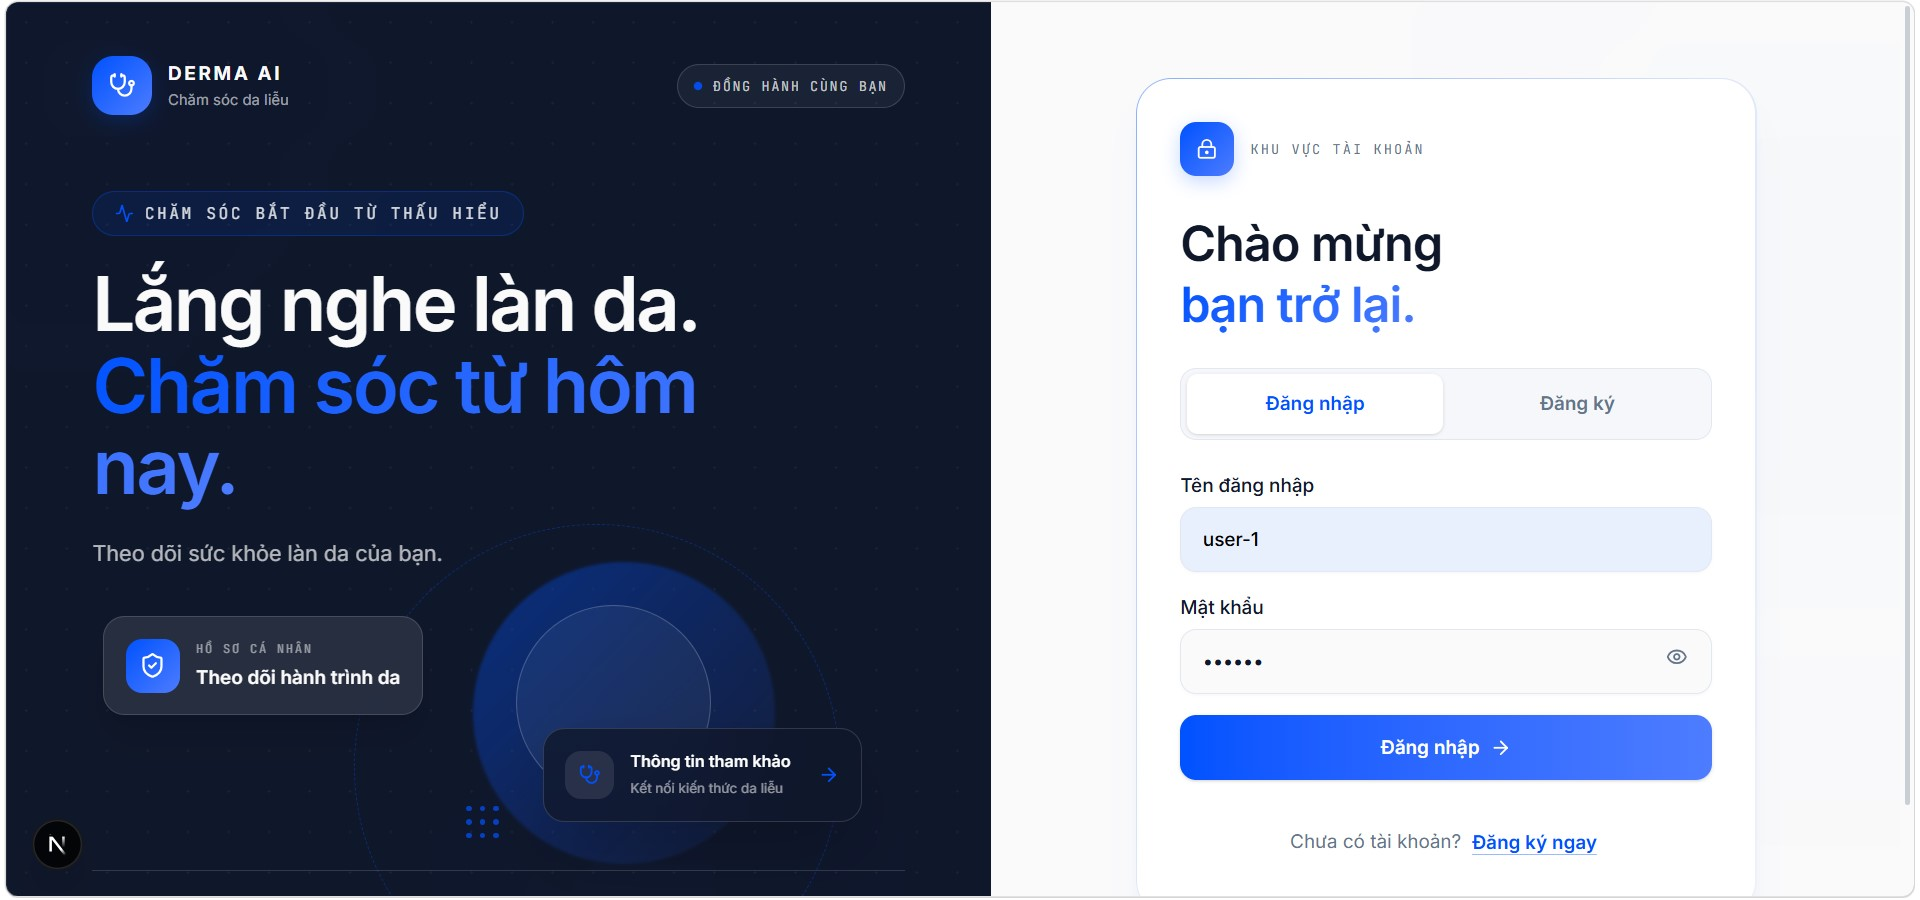
\includegraphics[width=0.95\linewidth,height=0.7\textheight,keepaspectratio]{chuong6/hinh/dang_nhap.jpg}
  \caption{Giao diện đăng nhập và đăng ký}
  \label{fig:gd-dang-nhap}
\end{figure}

\subsection{Bệnh nhân quản lý hồ sơ}

Một tài khoản bệnh nhân quản lý nhiều hồ sơ: bản thân, vợ/chồng, con và bố/mẹ. Cột trái liệt kê các hồ sơ kèm quan hệ và tuổi; cột phải hiển thị thông tin của hồ sơ đang chọn, gồm hai thẻ ``Thông tin'' và ``Kết luận''. Mục dị ứng, tiền sử và thuốc đang dùng được nhập theo từng dòng, như Hình~\ref{fig:gd-ho-so}. Dữ kiện dài hạn nhập ở đây được tác nhân AI dùng lại ở mọi lượt tư vấn của hồ sơ đó.

\begin{figure}[H]
  \centering
  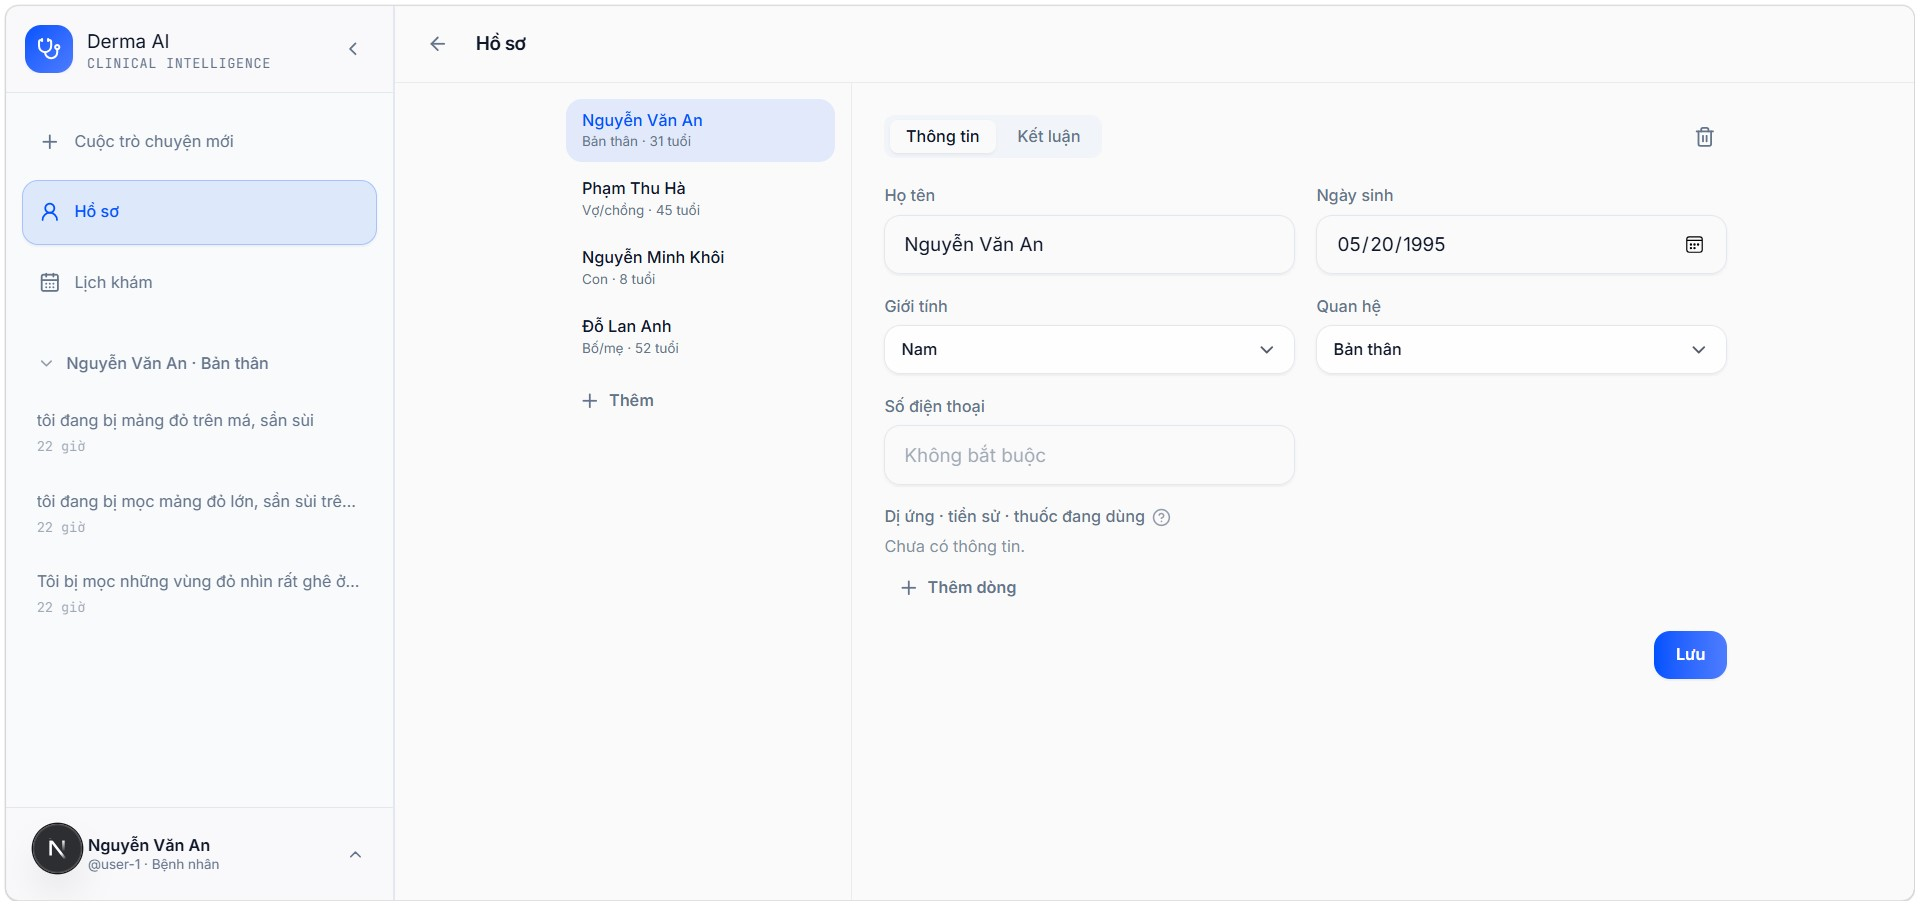
\includegraphics[width=0.95\linewidth,height=0.7\textheight,keepaspectratio]{chuong6/hinh/ho_so.jpg}
  \caption{Giao diện hồ sơ bệnh nhân với nhiều hồ sơ trong một tài khoản}
  \label{fig:gd-ho-so}
\end{figure}

\subsection{Bệnh nhân hỏi đáp với chatbot tiền chẩn đoán}

Khung chat hiển thị tiêu đề hội thoại, trạng thái của tác nhân và nút đính kèm. Câu trả lời chia thành ba phần: nhận định sơ bộ kèm độ tin cậy, những điều cần lưu ý thêm và khuyến cáo đi khám khi có dấu hiệu cần xử lý sớm. Nhãn ``Tiến trình suy luận'' ghi số bước mà tác nhân đã chạy cho lượt đó. Chân khung chat luôn hiển thị dòng nhắc kết quả chỉ mang tính tham khảo, như Hình~\ref{fig:gd-chat}.

\begin{figure}[H]
  \centering
  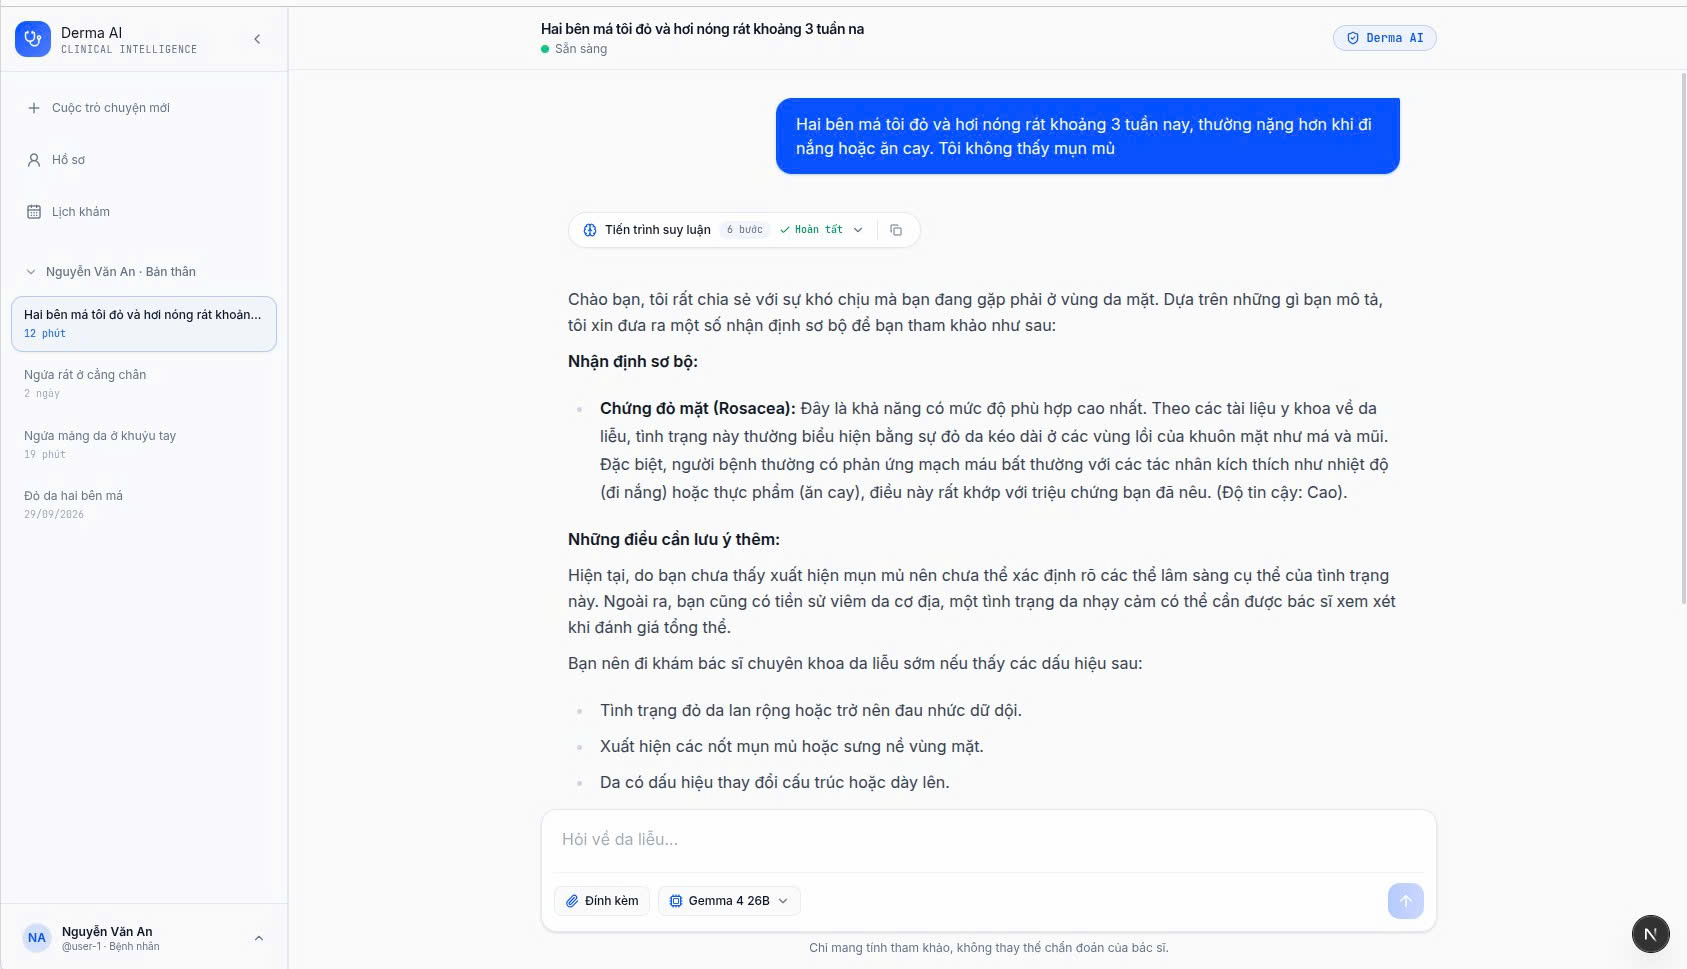
\includegraphics[width=0.95\linewidth,height=0.7\textheight,keepaspectratio]{chuong6/hinh/chat.jpg}
  \caption{Giao diện hỏi đáp với chatbot từ mô tả văn bản}
  \label{fig:gd-chat}
\end{figure}

Khi bệnh nhân gửi kèm ảnh tổn thương, tác nhân gọi thêm mô hình CNN trước khi trả lời. Nhận định sau đó viện dẫn đặc điểm nhìn thấy trên ảnh và giữ nguyên phần khuyến cáo, như Hình~\ref{fig:gd-chat-anh}. Số bước suy luận giảm so với lượt chỉ có văn bản vì tác nhân không phải hỏi lại mô tả.

\begin{figure}[H]
  \centering
  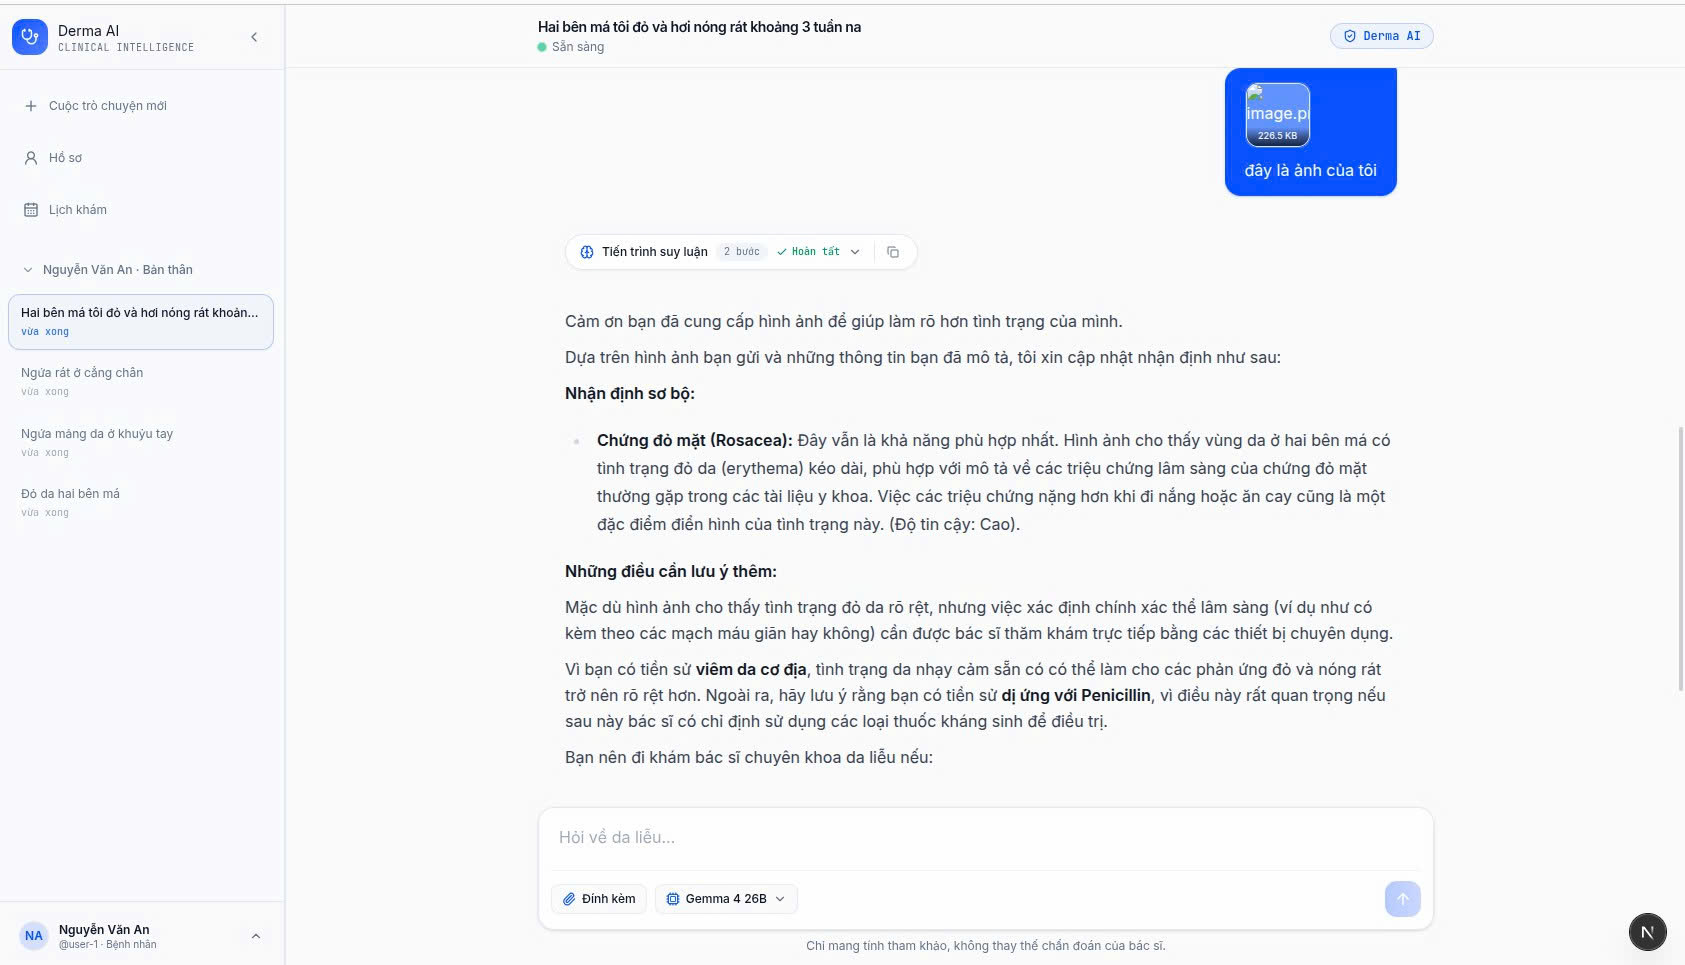
\includegraphics[width=0.95\linewidth,height=0.7\textheight,keepaspectratio]{chuong6/hinh/chat_co_anh.jpg}
  \caption{Giao diện hỏi đáp khi bệnh nhân gửi kèm ảnh tổn thương}
  \label{fig:gd-chat-anh}
\end{figure}

\subsection{Bệnh nhân yêu cầu tư vấn}

Trang lịch khám của bệnh nhân có hai thẻ: ``Đang theo dõi'' liệt kê các vùng da đang có vấn đề và ``Lịch hẹn'' liệt kê các lịch đã gửi. Mỗi dòng đang theo dõi có nút đặt lịch; hộp thoại đặt lịch yêu cầu chọn thời gian, lý do không bắt buộc. Sau khi gửi, dòng lịch chuyển trạng thái ``Chờ'' cho tới khi bác sĩ nhận.
% TODO: chèn ảnh màn hình "Lịch khám" của bệnh nhân (tab Đang theo dõi và hộp thoại đặt lịch).

\subsection{Bác sĩ tiếp nhận yêu cầu tư vấn và xem báo cáo tiền khám}

Trang chi tiết ca khám gom thông tin bệnh nhân, lý do khám, dữ kiện lâm sàng và gợi ý của AI trên cùng một cột, cột phải là kênh trao đổi với bệnh nhân. Mỗi dữ kiện có trạng thái xác nhận để bác sĩ đối chiếu trước khi dùng. Nút ``Xác nhận lịch'' chuyển lịch sang trạng thái đã hẹn và gán bác sĩ, như Hình~\ref{fig:gd-ca-kham}.

\begin{figure}[H]
  \centering
  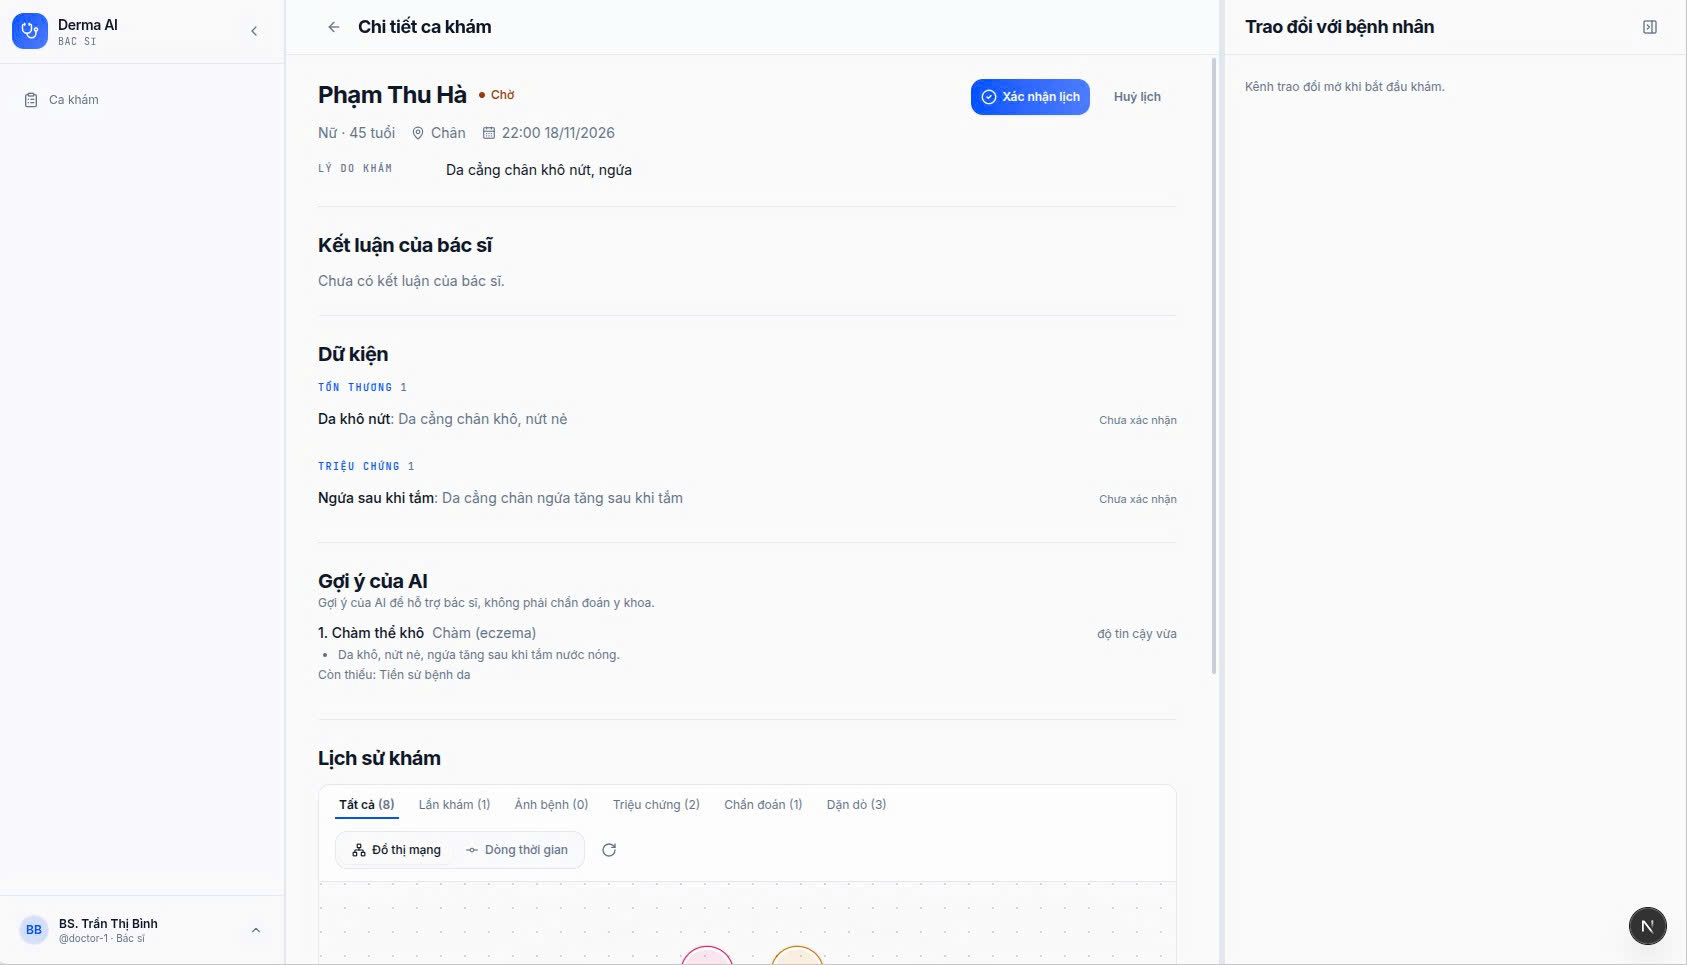
\includegraphics[width=0.95\linewidth,height=0.7\textheight,keepaspectratio]{chuong6/hinh/chi_tiet_ca_kham.jpg}
  \caption{Giao diện chi tiết ca khám: xác nhận lịch, dữ kiện lâm sàng và gợi ý của AI}
  \label{fig:gd-ca-kham}
\end{figure}

Phần lịch sử khám hiển thị theo hai dạng: đồ thị mạng và dòng thời gian. Đồ thị nối bệnh nhân với từng lần khám, triệu chứng, chẩn đoán và dự đoán của mô hình, như Hình~\ref{fig:gd-lich-su}. Bộ lọc phía trên giới hạn theo loại nút để bác sĩ chỉ xem phần cần đối chiếu.

\begin{figure}[H]
  \centering
  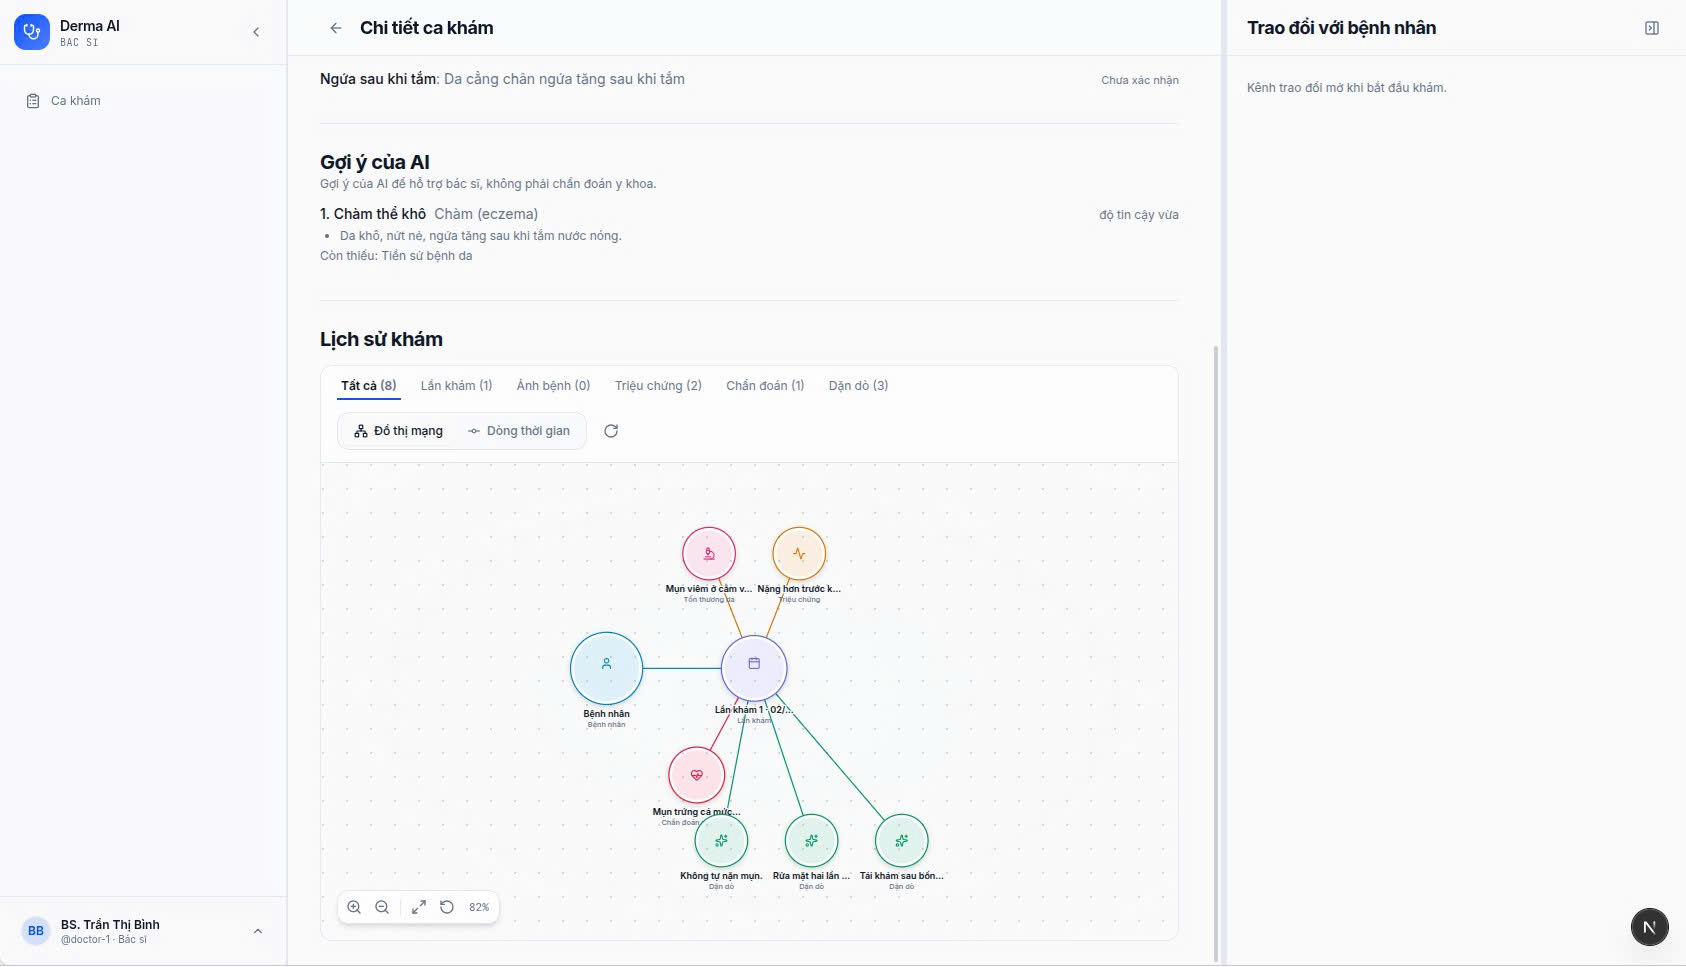
\includegraphics[width=0.95\linewidth,height=0.7\textheight,keepaspectratio]{chuong6/hinh/lich_su_kham.jpg}
  \caption{Lịch sử khám của bệnh nhân dạng đồ thị mạng}
  \label{fig:gd-lich-su}
\end{figure}

\subsection{Bệnh nhân và bác sĩ tư vấn video call}

Cuộc gọi video chạy trên WebRTC, ghép nối qua máy chủ TURN của hệ thống. Khung lớn hiển thị đối phương, khung nhỏ hiển thị camera của mình; ba nút phía dưới tắt micro, tắt camera và kết thúc cuộc gọi. Trạng thái cuộc gọi và thời điểm bắt đầu, kết thúc được lưu vào service tư vấn, như Hình~\ref{fig:gd-video-call}.

\begin{figure}[H]
  \centering
  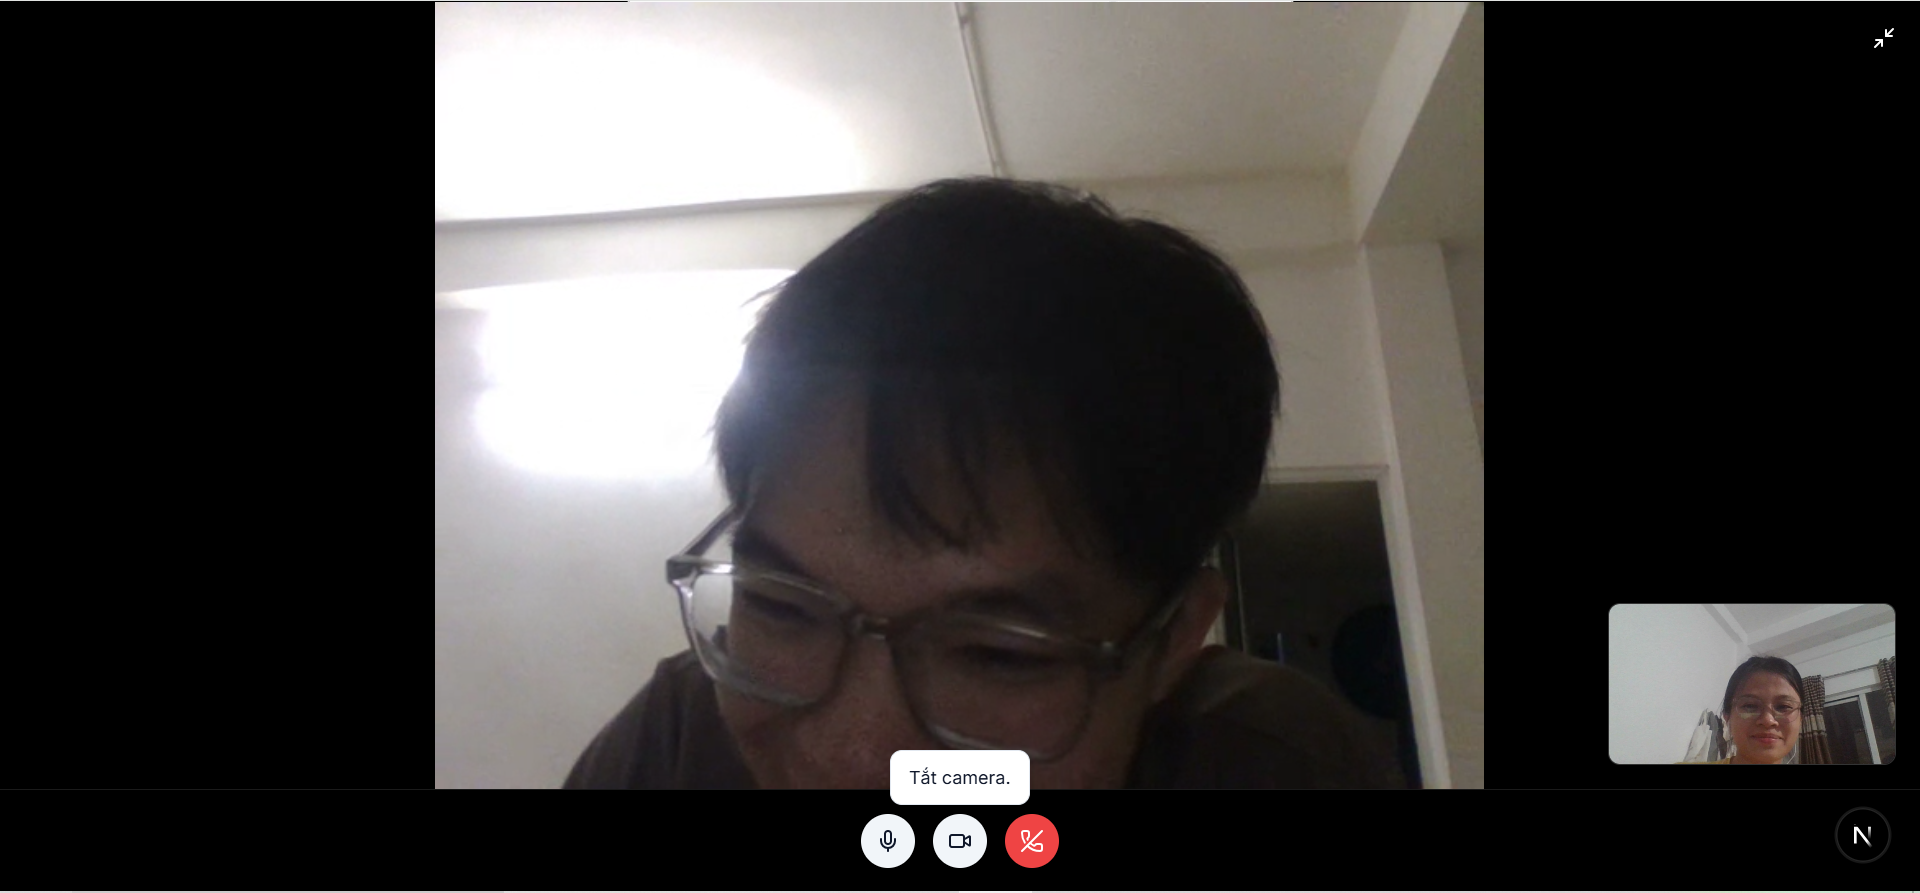
\includegraphics[width=0.95\linewidth,height=0.7\textheight,keepaspectratio]{chuong6/hinh/video_call.png}
  \caption{Giao diện cuộc gọi video giữa bác sĩ và bệnh nhân}
  \label{fig:gd-video-call}
\end{figure}

\subsection{Bác sĩ chốt báo cáo kết luận}

Sau khi thăm khám, bác sĩ nhập chẩn đoán, ghi chú và xác nhận lại các dữ kiện lâm sàng do AI đề xuất. Hệ thống lưu ảnh chụp báo cáo, mở kênh theo dõi sau khám 30 ngày và đóng lần khám. Nếu đánh dấu là ca tham khảo, dữ liệu được ẩn danh và nạp sang kho tri thức.
% TODO: chèn ảnh màn hình form chốt báo cáo kết luận của bác sĩ.

\subsection{Quản trị viên quản lý Knowledge Base}

Trang danh sách sách hiển thị tên sách, ngày tạo, số trang, dung lượng, tiến độ sáu bước và trạng thái xác nhận của từng sách, như Hình~\ref{fig:gd-sach}. Thanh tiến độ chia sáu ô tương ứng sáu bước xử lý; ô đổi màu theo trạng thái đã xác nhận, đang chờ, lỗi hoặc chưa chạy.

\begin{figure}[H]
  \centering
  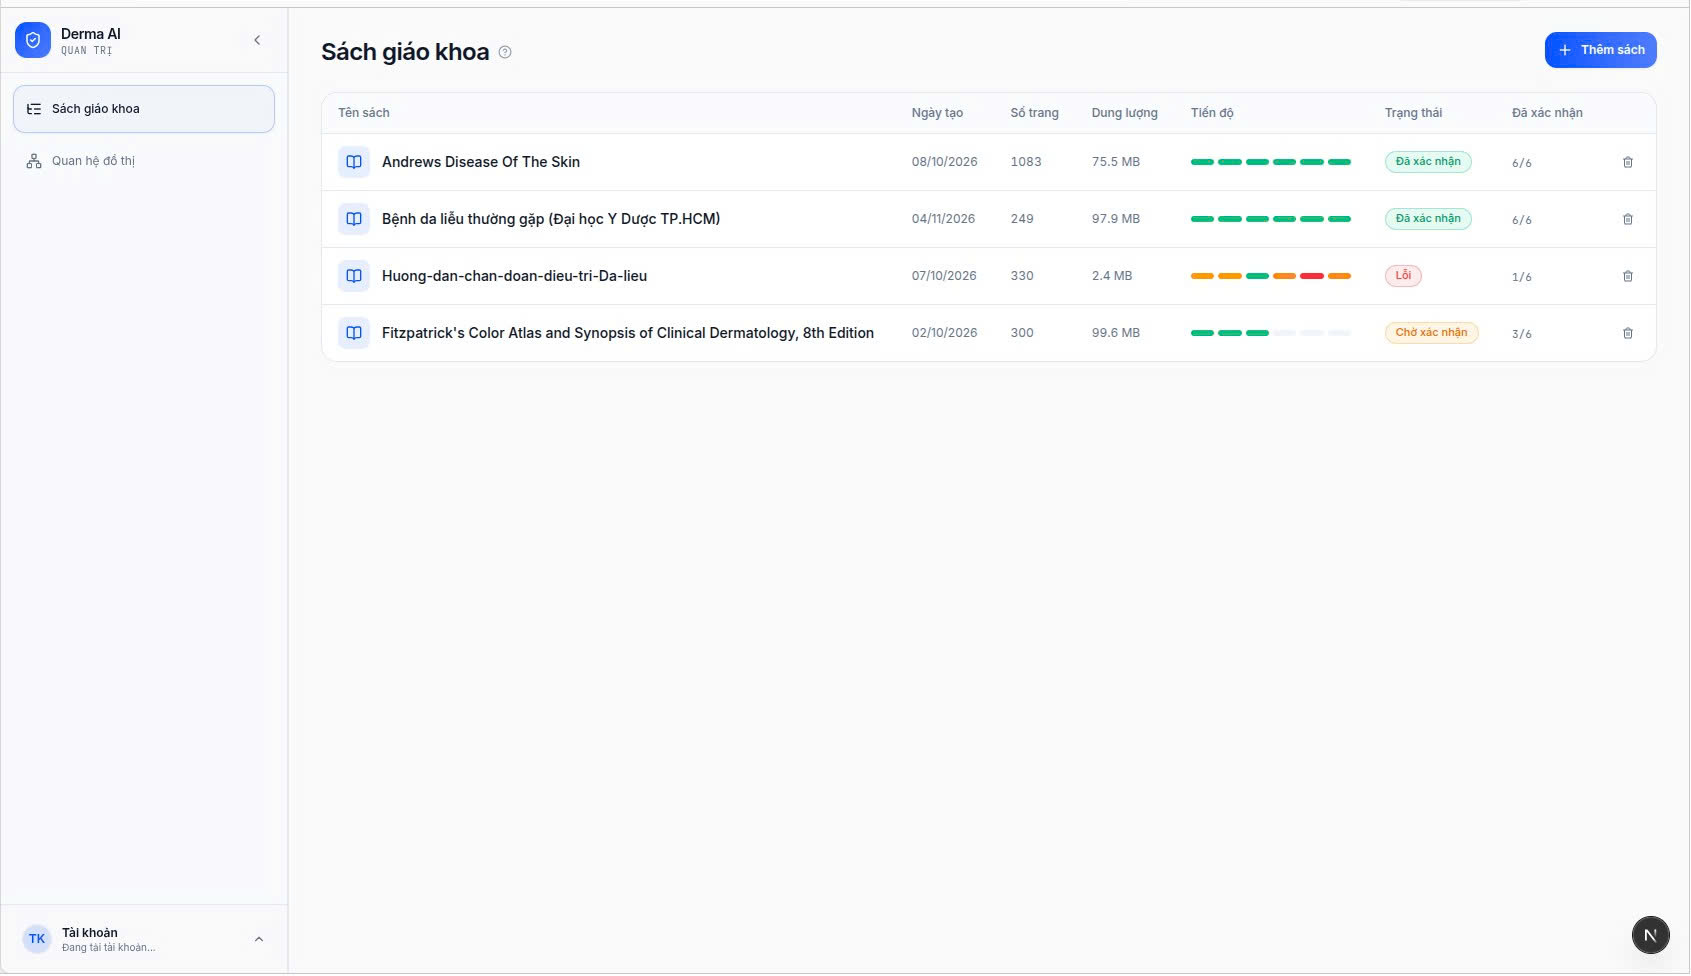
\includegraphics[width=0.95\linewidth,height=0.7\textheight,keepaspectratio]{chuong6/hinh/sach_giao_khoa.jpg}
  \caption{Danh sách sách giáo khoa kèm tiến độ sáu bước xử lý}
  \label{fig:gd-sach}
\end{figure}

Trang chi tiết một sách gồm dải sáu bước ở đầu và vùng nội dung theo bước đang chọn. Với bước trích quan hệ, vùng nội dung liệt kê từng quan hệ kèm hai đầu, câu trích trong sách và số trang in, có bộ lọc theo trạng thái khớp, như Hình~\ref{fig:gd-pipeline}. Cột phải hiển thị trang sách gốc để đối chiếu.

\begin{figure}[H]
  \centering
  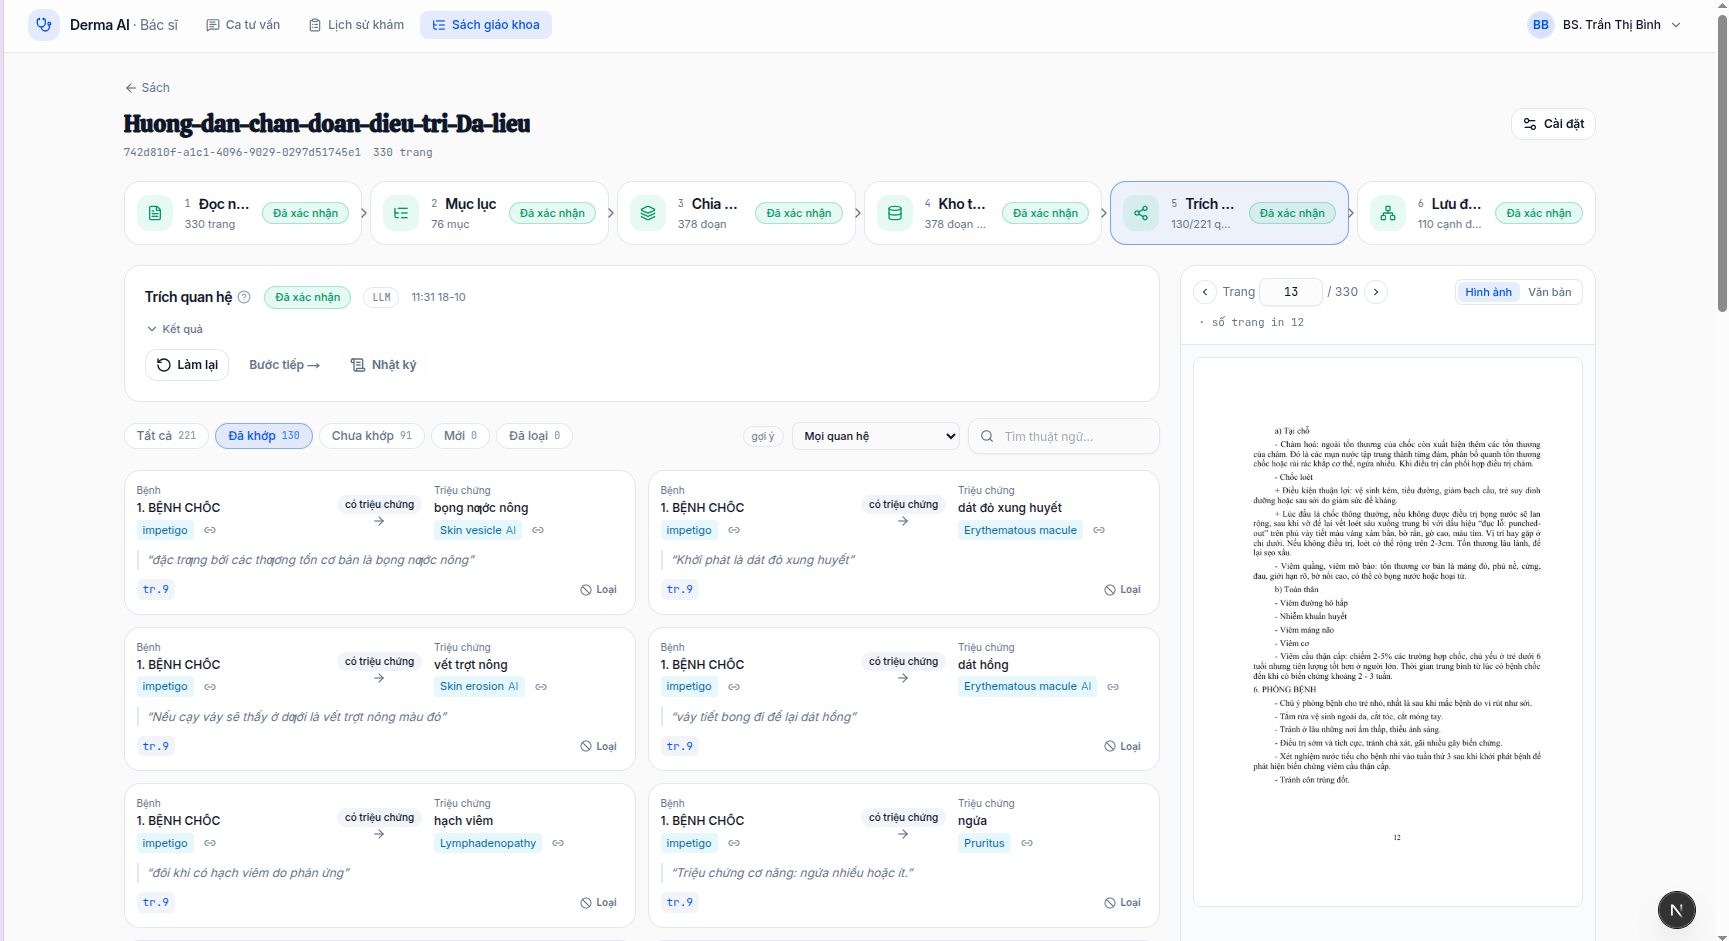
\includegraphics[width=0.95\linewidth,height=0.7\textheight,keepaspectratio]{chuong6/hinh/pipeline_sach.png}
  \caption{Trang chi tiết một sách: sáu bước xử lý và danh sách quan hệ trích xuất}
  \label{fig:gd-pipeline}
\end{figure}

Trang quản lý quan hệ của đồ thị tri thức liệt kê các loại quan hệ dùng khi trích xuất, mỗi dòng gồm tên hiển thị, nguồn thực thể, mã quan hệ, hai đầu và mô tả. Quản trị viên bật hoặc tắt từng loại quan hệ; bước trích quan hệ chỉ dùng các loại đang bật, như Hình~\ref{fig:gd-quan-he}.

\begin{figure}[H]
  \centering
  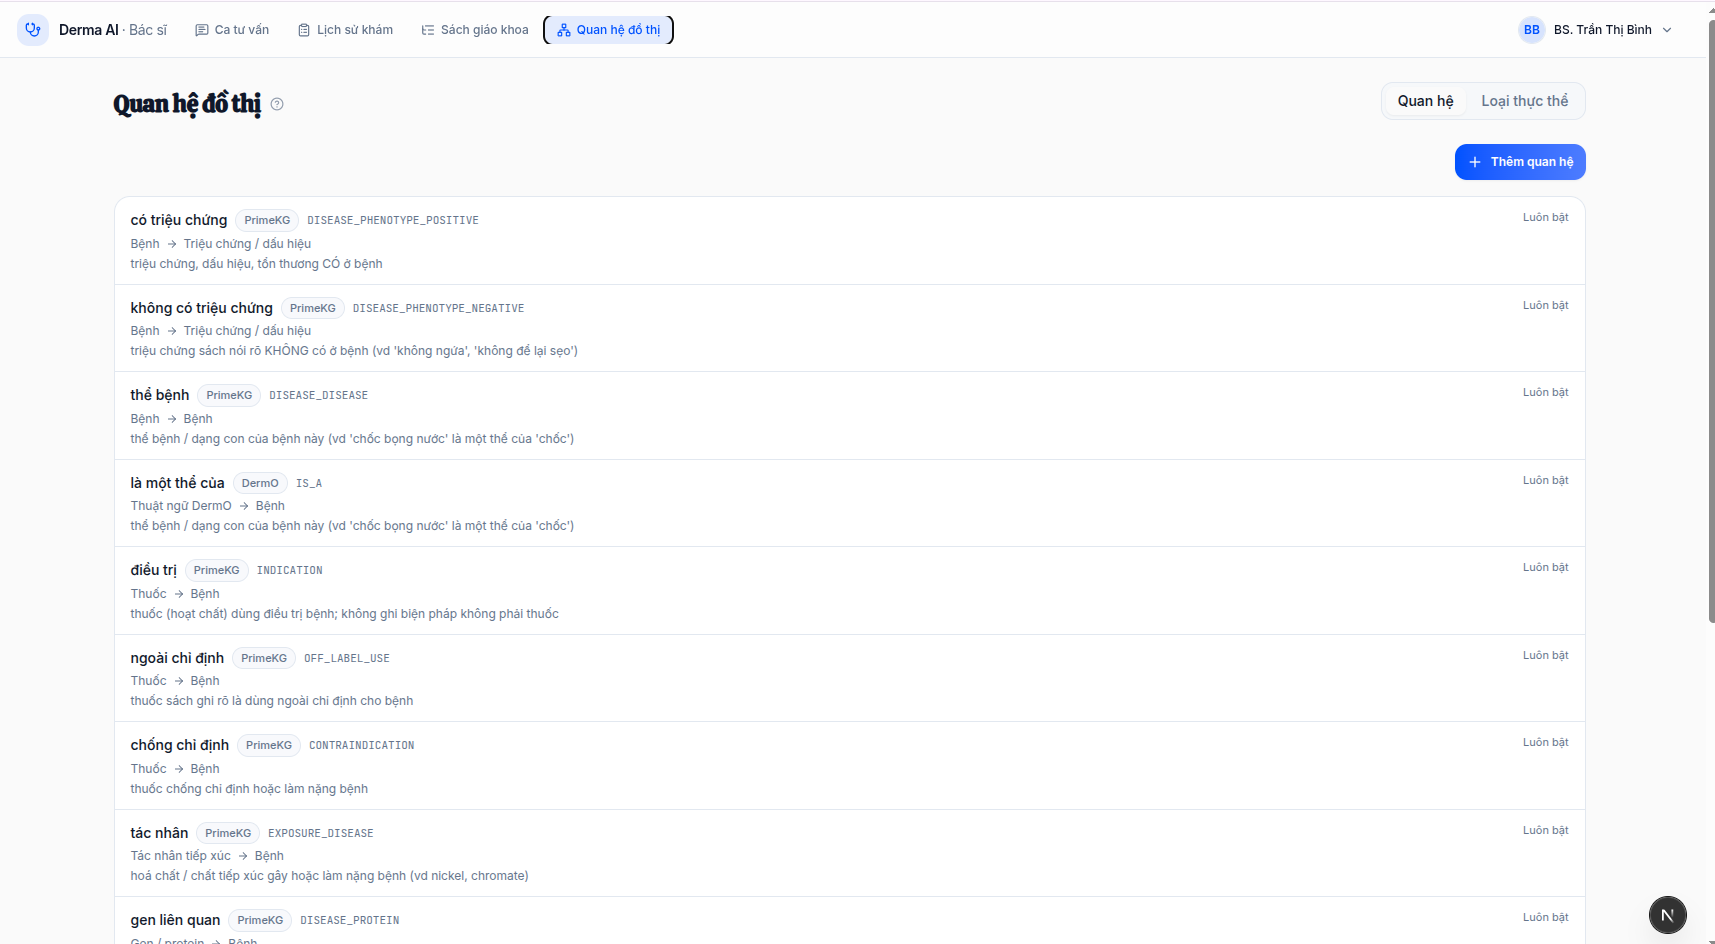
\includegraphics[width=0.95\linewidth,height=0.7\textheight,keepaspectratio]{chuong6/hinh/quan_he_do_thi.png}
  \caption{Trang quản lý quan hệ của đồ thị tri thức}
  \label{fig:gd-quan-he}
\end{figure}

\section{Kết luận}

Chương này trình bày cách cài đặt và kết quả giao diện của hệ thống. Phần cài đặt đi theo thứ tự: khởi động bảy container hạ tầng, tạo năm database, chạy sáu service cùng tiến trình worker, rồi chạy giao diện. Toàn bộ cụm cũng chạy được bằng Docker với bảy container dùng chung mạng nội bộ.

Phần giao diện lần lượt trình bày các màn hình theo sáu use case ở Chương 2, ở cả phía bệnh nhân, bác sĩ và quản trị viên. Hai màn hình chưa có ảnh chụp trong chương này là trang lịch khám của bệnh nhân và form chốt báo cáo kết luận của bác sĩ; phần mô tả luồng của hai màn hình nằm ở Chương 2.

Kết quả định lượng của mô hình phân loại ảnh và của luồng truy xuất tri thức đã trình bày ở Chương 3 và Chương 4.
